\section{Introduction}

\begin{figure}[t]
\centering
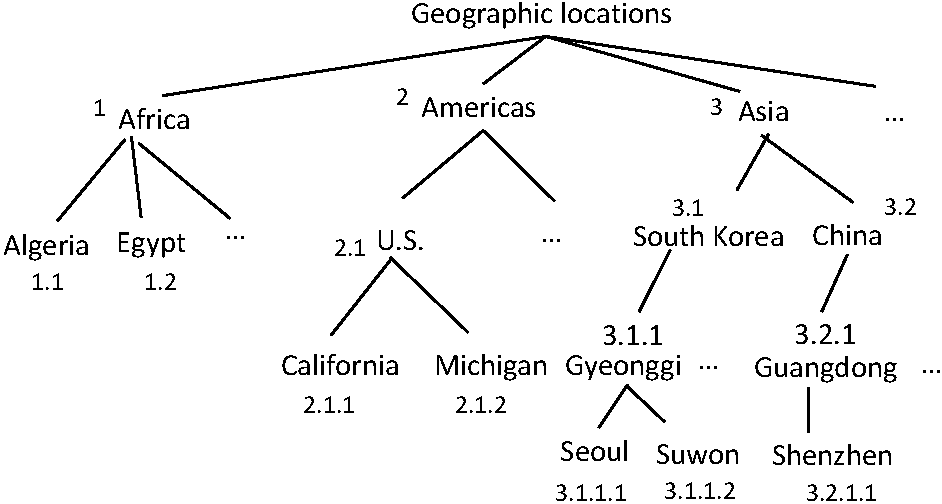
\includegraphics[width=0.45\textwidth]{figures/taxonomylabels}
 \caption{A toy example of taxonomy with labels}
\label{fig:taxonomyexample}
\end{figure}


\begin{figure}[t]
\centering
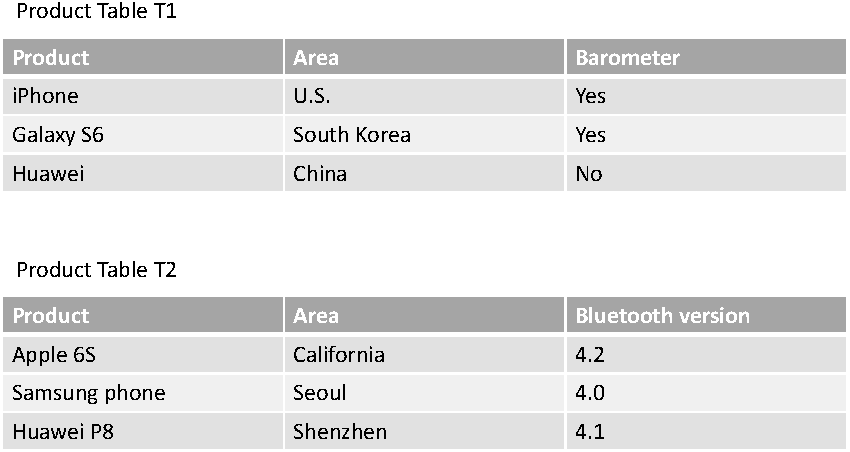
\includegraphics[width=0.45\textwidth]{figures/productexample}
 \caption{Two tables about the smart phones}
\label{fig:twotables}
\end{figure}


A string join, which finds all string pairs between two input collections, is an essential operation in many applications, such as  data integration \cite{conf/sigmod/Sarawagi04}, data cleansing \cite{conf/vldb/ArasuGK06,journals/www/LiJM06} and record linkage \cite{books/Winkler99}. In practice, a real-world entity has more than one representation in the data
collection; for example, the same address could be encoded using
different strings in different collections. Multiple representations
arise due to a variety of reasons such as misspellings
caused by typographic errors and different formatting conventions
used by data sources. Therefore, a string similarity join is an important operation for reconciling different
representations of an entity. A large number of different similarity functions such as Levenshtein distance~\cite{conf/sigmod/WangLF12},
Hamming distance~\cite{conf/spire/Kondrak05}, Episode
distance~\cite{conf/ijcai/CohenRF03}, Cosine
metric~\cite{journals/ipm/SaltonB88}, Jaccard
Coefficient~\cite{conf/icde/ChaudhuriGK06,conf/icde/LiLL08}, and Dice
similarity~\cite{conf/www/BayardoMS07} have been traditionally used in similarity joins. It is well known
that no single similarity function is universally applicable
across all domains and scenarios.


%  Conceptually, there are two cases of string joins: \textit{exact-joins} and \textit{approximate-joins}. Exact joins mean that two matching strings are exactly the same, while approximate joins tolerate certain difference between two strings and the similarity between two strings is measured by a similarity function, such as  Levenshtein distance~\cite{conf/sigmod/WangLF12},
%Hamming distance~\cite{conf/spire/Kondrak05}, Episode
%distance~\cite{conf/ijcai/CohenRF03}, Cosine
%metric~\cite{journals/ipm/SaltonB88}, Jaccard
%Coefficient~\cite{conf/icde/ChaudhuriGK06,conf/icde/LiLL08}, and Dice
%similarity~\cite{conf/www/BayardoMS07}.

In recent years, we have witnessed the emergence of various efforts to enhance the effectiveness of string similarity joins by using synonyms \cite{conf/sigmod/LuLWLW13,conf/icde/ArasuCK08,conf/cpm/BarbayGMR06,conf/vldb/ArvindSR09}.
The traditional similarity functions consider only syntactic similarities, e.g., number of common
words or $q$-grams. But there are many important cases where syntactically different
strings can represent the same real-world object. For example,
``\textsf{Bill}'' is a short form of ``\textsf{William}'', and ``\textsf{ICDE}'' is an abbreviation of  ``\textsf{International Conference on Data Engineering}''.  Given two collections of strings,  synonym-based similarity functions can utilize the available synonyms to find string pairs which are semantically similar. While those methods improve the effectiveness of string joins, a synonym dictionary does not contain information such as
``\textsf{Helsinki is a city of Finland}'', or `\textsf{`Apple 6 Plus is a new model of iPhone}''. Still, term pairs such as ``\textsf{Helsinki}'' and ``\textsf{Finland}'', ``\textsf{Apple 6 Plus}'' and ``\textsf{iPhone}''  have strong semantic correlations.


In this paper, we assume that we already have complete
information of these IS-A relations, i.e. \textit{taxonomy}, and we will focus on how
to efficiently perform a string join by utilizing the taxonomy, and how to optimize the index structure
for this purpose.  Taxonomies are sets of IS-A hierarchies, which identify the relations between different concepts. The IS-A relationship
is a transitive closure of the concept-instance relationship.
For example, if ``\textsf{kitten}'' is an instance of ``\textsf{cat}'', and
``\textsf{cat}'' is an instance of ``\textsf{pet}'', then ``\textsf{kitten}'' is an instance
of ``\textsf{pet}''. If we treat each term as a node, and create
for each (concept, instance) pair, an edge from the concept
to the instance, then we can think of the taxonomy as a tree or forest. For any node that representing a term,
the IS-A relation could be any descendant of it in the tree. Figure
1 gives an example of a toy geographical taxonomy tree.

%For example, the (Guangdong, Shenzhen) is a (concept, instance) pair and (Shenzhen, China) has the IS-A relation, as Shenzhen is a city in China.



To support string joins with taxonomy in databases, we can extend the SQL language by adding a new predicate ``IS-A''. For example,
consider two tables in Figure \ref{fig:twotables}, which contain the information about the products of cellphones.  Consider the following SQL script:

\vspace{2mm}

\noindent \textsf{Select T1.price, T2.price} \\
\noindent \textsf{ From T1 and T2} \\
\noindent   \textsf{Where T2.product \textbf{IS-A} T1.product and T2.area \textbf{IS-A} T1.area}

 \vspace{2mm}


\noindent which selects the prices of phones from two tables by performing the two IS-A joins against ``\textsf{product}'' and ``\textsf{area}'' columns (e.g. ``\textsf{Galaxy S6}'' is a model of ``\textsf{Samsung}'' in the product column and ``\textsf{Seoul}'' is a city of ``\textsf{South Korea}'' in the area column).


The IS-A predicate requires the two terms to be ancestor-descendant relationship. But it cannot capture the sibling relation between terms. For example, in Figure \ref{fig:taxonomyexample}, California and Michigan have no IS-A relation, but they are similar in the sense that both are states in America. Therefore, we propose the new function called Taxonomy-similarity (TS) to quantify the similarity of strings with the taxonomy tree. Generally speaking,  the bigger the similarity between two terms, the closer they are in the taxonomy tree.  For example, the similarity between California and Michigan is greater than that between California and Seoul.


The TS function captures the semantic hidden in the taxonomy tree, but it requires that one string record can only match one term in the taxonomy. In some cases, a string may match multiple term together. For example, one string ``California, U.S. '' match two terms in the taxonomy. Therefore, in this work, we further extend the TS function to propose a new function which consider the substring matching for the taxonomy.

 Given two collections of strings $S$ and $T$, a baseline algorithm is to perform nested-loop joins for each pair of strings from each collection. Clearly, this method is inefficient. In this paper, we develop a new index for $S$ and $T$ with taxonomy node inverted lists with prefix labels, then we first perform the prefix join for inverted list, and then perform Cartesian join for the strings and obtain the final results. We can prove that our algorithm is optimal in the sense that each output is part of answers.



Many real-world applications require solving a similarity join problem where one is interested in all pairs of objects whose
similarity is above a specified threshold. This trend is fueled in part by the
recognition that many application scenarios can significantly
benefit from the identification of similarities in the data. One
of the most useful similarity-aware data analysis operations is
the Similarity Join (SJ), which retrieves all data pairs whose
distances are smaller than a predefined threshold $\epsilon$. Similarity
joins have been studied and extensively used in multiple application
domains, e.g., record linkage, data cleaning, multimedia
applications, sensor networks, marketing analysis, etc. In this paper, we study how to utilize the taxonomy with approximate string joins.



The existing function the brute-force algorithm that enumerates every string pair and checks whether the two strings in the pair are similar is rather expensive. To alleviate this problem, many algorithms have been proposed in the recent two decades. One widely-adopted technique employs a filter-verification framework, which includes two steps: (1) Filter step: devising effective filtering algorithms to prune large numbers of dissimilar pairs and generating a set of candidate pairs; and (2) Verification step: verifying each candidate pair by computing
the real similarity and outputting the final results. Filtering algorithms in the first step play an important role
in the framework. Most of existing filtering algorithms employ a signature-based technique, which generates signatures for each string such that if two strings are similar, their signatures must have overlaps. Thus the signature-based technique can prune string pairs that have no common signature.

Recently many filtering techniques have been proposed, e.g., count filtering [8,13,18], length filtering [8,14], position
filtering [25,27], prefix filtering [4] and content filtering [25]. As prefix filtering is the most effective filtering technique,
many algorithms have been proposed to optimize prefix filtering for different similarity metrics, e.g., AllPair [2],
PPJoin [27], EDJoin [25], QChunk [17], VChunk [24], AdaptJoin [23]. There are also many other signature schemes, e.g., PartEnum [1],
PassJoin [14], FastSS [20].

Unfortunately, these algorithms are not easily extended to process taxonomy. Because all the existing methods are based on the observation that two strings are similar only if their signatures overlap. But this is not true for taxonomy, because two strings may have IS-A relation without any common tokens (signatures).

The leave behind two intriguing questions:

1. How to efficient process string joins with taxonomy? And for multiple joins.


2. How to process the similarity joins and multiple-way similarity joins?  This question becomes increasingly urgent nowadays with the arrival of big data.

When we tried to apply these known technologies in our taxonomy environment, however, we encounter a few critical challenges, summarized as below:

\noindent \textit{Taxonomy signature}

\noindent \textit{Taxonomy update}

%\begin{problem}(String measure with taxonomy). Given two strings $s_1$ and $s_2$ and a taxonomy $T$, how to measure the similarity between $s_1$ and $s_2$ based on T?
%\end{problem}
%\begin{problem}(String joins with taxonomy). Given a string $p$$\in$
%$\Sigma^*$, an integer k, and a synonym set $\mathbb{R}$,  .
%\end{problem}




\subsection{Novelty and contributions}


\smallskip


Our contributions are as follows.

\noindent \textbf{Introduction of string joins with taxonomy}. We introduce a new problem to utilize the taxonomy for the string joins in databases, which has application in data integration and data cleansing.

\noindent \textbf{Optimal algorithms for exact-joins} We develop an inverted list introduce an algorithm for multiple string joins.

\noindent \textbf{Novel algorithms for approximate-joins}

\noindent \textbf{Generality and variations}  We introduce a novel algorithm for incrementally updating taxonomy. Our merging algorithm allows us to incorporate new correlations introduced over a subset of tuples into
the correlations already present in the database, without recomputing the existing results.


Finally, we perform experiments to evaluate our results and show the benefits of proposal algorithms.


\smallskip

The rest of this paper is organized as follows. Section 2
provides the necessary definitions, formulates . Section
3 includes our algorithm for exact joins with taxonomy. In Section 4, we study
the approximate string join, proposing our solution, analyzing its approximation
ratio, and presenting our similarity join algorithms.
Our experiments are presented in Section 5. Finally,
Section 6 concludes with a discussion about future work.
